\section{Auswertung}
\label{sec:Auswertung}
Die Fehler der Widerstände $R$, Kapazitäten $C$ und der Induktivitäten $I$ betragen jeweils $\pm \qty{0.2}{\percent}$. Das Verhältnis $R3/R4$ am Potentiometer
weist einen Fehler von $\pm \qty{0.5}{\percent}$ auf und die verstellbaren Widerstände eine Ungenauigkeit von $\pm \qty{3}{\percent}$. 

\subsection{Wheatstonesche Brücke}
\label{subsec:wheat_aus}
\begin{table}[H]
  \centering
  \caption{Messwerte der Wheatstoneschen Brücke.}
  \label{tab:wheat}
  \sisetup{table-format=3.0}
  \begin{tabular}{S[table-format=4.0] S S S[table-format=3.2]}
   \toprule
    {$R_2 $[\si{\ohm}]} & {$R_3$ [\si{\ohm}]} & {$R_4 $[\si{\ohm}]}&{ $R_x = Wert10$[\si{\ohm}]}\\
   \midrule
   332 & 420 & 580 & 240.41 \\
   500 & 325 & 675 &  240.74\\
   1000 & 194 & 806 &  240.70\\
   \bottomrule
  \end{tabular}
\end{table} 

Für die Berechnung des Mittelwerts 
\begin{equation*}
  R_{\text{xm}} = 240.62
\end{equation*}
und der Standardabweichung
\begin{equation*}
  \sigma_{\text{xm}} = 0.14
\end{equation*}
von $R_x$ wurde das Pythonmodul Numpy \cite{numpy} herangezogen.
Der Fehler des Mittelwerts berechnet sich analog zu
\begin{equation*}
  \Delta R_{\text{xm}}= 0.08.
\end{equation*}

\noindent Die Fehlerfortpflanzung nach Gauß, gemäß
\begin{equation*}
  \Delta f = \sqrt{\biggl(\frac{\partial f}{\partial x}\biggr)^2\cdot (\Delta x)^2 + \biggl(\frac{\partial f}{\partial y}\biggr)^2\cdot (\Delta y)^2 +
  \cdots + \biggl(\frac{\partial f}{\partial z}\biggr)^2\cdot (\Delta z)^2}
\end{equation*}
wird im folgenden auch mithilfe des Pythonmoduls Numpy \cite{numpy} berechnet.
\subsection{Kapazitätsmessbrücke}
\label{subsec:kap_aus}
\begin{table}[H]
  \centering
  \caption{Messwerte der Kapazitätsmessbrücke.}
  \label{tab:kap}
  \sisetup{table-format=3.0}
  \begin{tabular}{c S S S S S[table-format=3.2] S[table-format=3.2]}
   \toprule
  &{$C_2$ [\si{\nano\farad}]}&{$R_2$ [\si{\ohm}]} & {$R_3$ [\si{\ohm}]} & {$R_4$ [\si{\ohm}]}&{$R_x$ [\si{\ohm}]} & {$C_x$ [\si{\nano\farad}]}\\
  \midrule
   Wert 9 & 992 & 192 & 691 & 309 & 443.6 & 429.36\\
   Wert 1 & 992 & 0 & 605 & 395 & 647.67 & 0 \\
   \bottomrule
  \end{tabular}
\end{table}


  

\subsection{Induktivitätsmessbrücke}
\label{subsec:indu_aus}
\begin{table}[H]
  \centering
  \caption{Messwerte der Induktivitätsmessbrücke.}
  \label{tab:indu}
  \sisetup{table-format=3.0}
  \begin{tabular}{c S S S S S[table-format=3.2] S[table-format=3.2]}
  \toprule
  &{$L_2$ [\si{\milli\henry}]}&{$R_2$ [\si{\ohm}]} & {$R_3$ [\si{\ohm}]} & {$R_4$ [\si{\ohm}]}&{$R_x$ [\si{\ohm}]} & {$L_x$ [\si{\milli\henry}]}\\
  \midrule
  Wert 17& 27.5 & 59 & 609 & 391 & 91.90 & 42.83\\
  \bottomrule
  \end{tabular}
\end{table}
Die Fehler der 

Wien-Robinson-Brücke
\begin{table}[H]
  \centering
  \caption{Messwerte der Spannung bei variabler Frequenz.}
  \label{tab:mess}
  \begin{tabular}{S[table-format=5.0] S[table-format=1.2]}
    \toprule
    {$\nu \mathbin{/} \si{\second\tothe{-1}}$} & {$U_Br \mathbin{/} \si{\volt}$}\\
    \midrule
    20    & 3.0  \\
    50    & 2.9  \\
    100   & 1.9  \\
    200   & 0.4  \\
    220   & 0.2  \\
    230   & 0.1  \\
    240   & 0.02 \\
    250   & 0.09 \\
    260   & 0.19 \\
    280   & 0.36 \\
    300   & 0.44 \\
    350   & 0.8  \\
    400   & 1.1  \\
    500   & 1.5  \\
    750   & 2.2  \\
    1000  & 2.5  \\
    2000  & 3.0  \\
    3000  & 3.1  \\
    4000  & 3.2  \\
    5000  & 3.2  \\
    7500  & 3.2  \\
    10000 & 3.2  \\
    15000 & 3.1  \\
    20000 & 3.0  \\
    \bottomrule
  \end{tabular}
\end{table}

\begin{figure}
  \centering
  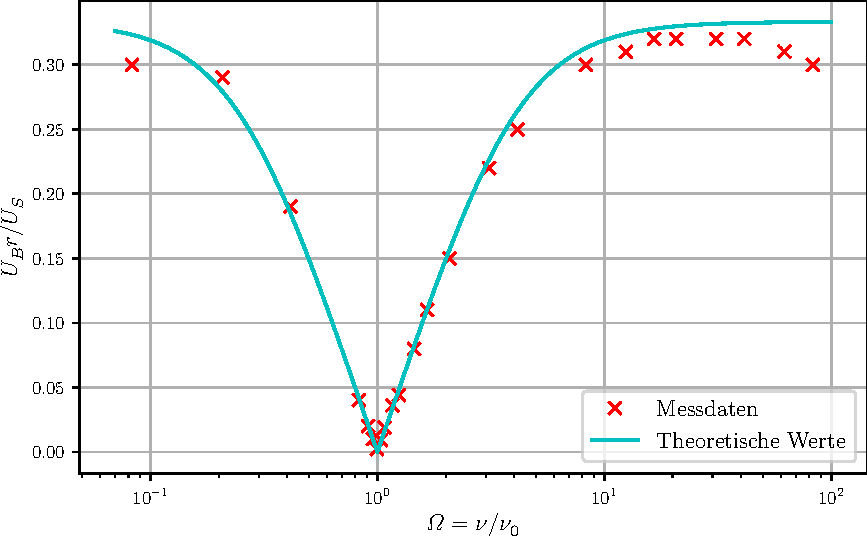
\includegraphics{plot.pdf}
  \caption{keine Ahnung wie man das nennt...}
  \label{fig:wrb-plot}
\end{figure}



%   aaaaaaaaaaaaaaaaaaa
%   R_x  [240.4137931  240.74074074 240.69478908]
%   Mittelwert  240.61644097535827
%   Standardabweichung 0.14451645518791226
%   Fehler des Mittelwertes  0.08343661430507164
%   Abw theorie 0.68+/-0.03
%   bbbbbbbbbbbbbbbbbbb
%   Wert 9
%   R2 192.0+/-0.4 R3 691.0 R4 309.0
%   Rx 429.36+/-2.31
%   Abw theorie -7.64+/-0.50
%   Cx (4.4360+/-0.0239)e-07
%   Abw theorie 2.28+/-0.55
%   Wert 1
%   R2 0 R3 605.0 R4 395.0
%   Rx 0.00+/-0
%   Cx (6.4767+/-0.0349)e-07
%   Abw theorie -1.87+/-0.53
%   cccccccccccccccccccc
%   R2 59.00+/-0.12 R3 609.0 R4 391.0
%   Rx 91.90+/-0.49
%   Abw theorie -1.87+/-0.53
%   Lx (4.2832+/-0.0231)e-02
%   Abw theorie 2.35+/-0.55
%   ddddddddddddddddddddd
%   R2 500.0+/-1.0 R3 291+/-9 R4 1000+/-30
%   Rx 145.50+/-6.18
%   Abw theorie 55.37+/-6.60
%   Lx (6.5475+/-0.1973)e-02
%   Abw theorie 56.45+/-4.71
%   eeeeeeeeeeeeeeeeeeeee
%   U2 0.1341640786499874
%   Klirrfaktor 0.01341640786499874